\clearpage
\subsection{Study IV --- the finite-sector diffusion closure}\label{sec:study4}

\begin{sloppypar}
Study III added even-parity angular modes inside each angular segment and
changed the body closure. This section assesses the branch that keeps the
PSN idea in its literal form: the transport equation is reduced, per finite
angular cell, to a diffusion-type equation whose coefficients are the exact
second-moment tensor of the directions in that cell, and the resulting
systems are assembled over space exactly as a diffusion calculation would
be. The branch reduces that tensor two ways, at equal cost. At azimuthal degree
$A$ each sector carries $K{=}A{+}1$ angular unknowns either way: in the closure
\texttt{sector\_diffusion} they are the $A{+}1$ Gauss directions of the sector,
each retaining its own tensor, and in \texttt{sector\_average} they are the cell
mean plus $A$ local azimuthal modes ($A{=}0,\ldots,4$). The direction-wise
\texttt{sector\_diffusion} is the closure of record in this section and the
default of the driver named below, at $A{=}3$ unless the input asks otherwise;
\texttt{sector\_average} is kept as the comparison at equal degrees of freedom.
The quarter-core matrices, the fission maps and Table~\ref{tab:study4-checker-sector}
were measured with the direction-wise closure;
Table~\ref{tab:study4-checker-average} repeats the same checkerboard grid with the
cell-average one, point for point, and Table~\ref{tab:study4-closure-ratio} reports
the ratio of the two eigenvalue errors at each of the 189 points measured both ways.
The one exception among the measurement tables is the set of six wide $S\times M$
matrices of Table~\ref{tab:study4-assembly}, which is still the archived
cell-average sweep; its direction-wise re-sweep was running while this was written
and had converged at 213 of the 458 points it plans --- every point of the published
checkerboard grid, 73 of the 200 wide checkerboard points and 26 of the 144 assembly
points, all merged into the same two data files as \texttt{closure=sector\_diffusion}
rows beside the archived ones, so no table mixes the two closures. The ten \texttt{strict\_phase\_space} rows kept in the same
checkerboard data file are neither closure: they insert the exact sector tensor into
the original four-mode body and face-average matching, and are quoted only where the
published valley is located. Both closures are selected from the input file
(\texttt{angular.model: generic}, \texttt{angular.closure: sector\_diffusion} or
\texttt{sector\_average}, \texttt{angular.azimuth\_degree},
\texttt{angular.polar\_degree}, \texttt{angular.slope\_space}); the driver
\texttt{scripts/sector\_diffusion\_benchmark.py} reproduces every point
below, \texttt{scripts/study4\_closure\_report.py} rebuilds the two checkerboard
matrices, their point-by-point ratio table and the paired data file
\texttt{paper/data/study4\_closure\_pairs.csv} from the same records,
\texttt{scripts/study4\_closure\_cost.py} measures the matched cost pairs of
Table~\ref{tab:study4-closure-cost}, \texttt{scripts/study4\_uniform\_grid.py} runs
and merges the re-sweep, and \texttt{scripts/study4\_core\_report.py} rebuilds the
core tables from the recorded run logs. The same closure is written up on its own terms in
\texttt{paper/sector\_method.tex} --- even-parity reduction, sector tensors, the
counterexamples that bound the word ``exact'', the test-problem inventory and the
cost records --- which compiles and reads independently of this paper and shares its
generated tables.

\end{sloppypar}

\paragraph{Formulation.}
Inside a material-constant node, decomposing the angular flux into its even
and odd parts under $\boldsymbol{\Omega}\rightarrow-\boldsymbol{\Omega}$
gives, for isotropic scattering and fission, the exact relation
$\psi^{-}=-(\boldsymbol{\Omega}\cdot\nabla u)/\Sigma_t$ for the even-parity
flux $u$. Eliminating $\psi^{-}$ yields, for each retained direction,
\begin{equation}
-\nabla\cdot\!\left(\frac{\boldsymbol{\Omega}\boldsymbol{\Omega}^{\mathsf T}}{\Sigma_t}\nabla u\right)
+\Sigma_t u = q ,
\label{eq:study4-even}
\end{equation}
with the vacuum boundary condition carrying $|\boldsymbol{\Omega}\cdot\mathbf{n}|u$
and specularly reflected directions sharing the trace value on the reflecting
face. Equation~\eqref{eq:study4-even} is discretised in space by continuous
biquadratic Lagrange nodes, with the body diffusion term, the normal current
across material interfaces and the vacuum term taken from one weak form, so
no separate face-current model is introduced. Scattering and fission are
projected onto nine orthogonal spatial moments per material node. Azimuth is
split into $M$ sectors per half-plane, each carrying $A{+}1$ Gauss
directions; polar angle uses Gauss nodes ($I/2$ per half-axis) or the
existing three-point TY3 rule. The tensor
$\langle b_a\,\boldsymbol{\Omega}\boldsymbol{\Omega}^{\mathsf T}b_b\rangle/\Sigma_t$
is integrated analytically over each finite cell, and its $xy$ component is
retained, so two directions in one sector that differ only in sign of
$\Omega_x\Omega_y$ are not collapsed. For the mirrored quadrant-symmetric
assemblies, complementary azimuths are solved once and applied by the spatial
transpose.

\begin{sloppypar}
Two reductions were verified algebraically rather than numerically. Setting
\texttt{angular.node\_response: true} rewrites the same weak form as a shared
face-trace system, $R=\mathsf{K}_{II}^{-1}\mathsf{K}_{IB}$,
$\mathsf{T}_B=\mathsf{K}_{BB}-\mathsf{K}_{BI}R$,
$\mathbf{g}_B=\mathbf{f}_B-R^{\mathsf T}\mathbf{f}_I$, with the nodal interior
recovered afterwards. Because $\mathsf{K}_{II}$ is block-diagonal per node,
this is an exact elimination of the interior degrees of freedom, and the
repository checks it two ways: on a three-material rectangle, in four different
spatial and angular subspaces and two of them in the reflection-invariant
subspace, the condensed trace solve reproduces a direct sparse solve of the full
angular matrix to $2\times10^{-11}$, and on the strong checkerboard the eliminated and direct
systems give the same eigenpair to a relative tolerance of $2\times10^{-9}$
with the spatial and angular test spaces unchanged
(\texttt{tests/test\_sector\_diffusion.py}). Changing $A$, by contrast, changes the test space, and its effect
is measured below. A second check concerns what a finite angular closure can
and cannot achieve: for a purely absorbing slab, the map from an incident
angular profile $g(\mu)$ to the exit profile is $e^{-T/\mu}g(\mu)$, which is
injective on angular functions, so any fixed number of retained angular
moments admits two incident profiles with identical moments and different
outgoing states. A reflective slab with a cosine source gives a response
coefficient of $\pi/4$ when the direction-wise solution is averaged after the
fact and $3/4$ when the diffusion tensor is averaged over angle first. Exact
transfer between nodes therefore requires a continuous face function, and
$S$ and $M$ then only partition the phase space. This is the sense in which
the closure is ``strict'': the algebra is exact up to the chosen finite
spatial and angular spaces, and no additional face-current model is hidden in
the assembly.

\end{sloppypar}

\paragraph{The diagonal valley of the square checkerboard.}
On the one-group square checkerboard of the original paper the published PSN
errors change sign along a diagonal valley whose position moves with $S$: at
$I{=}30$ the strong-absorber row $S{=}2$ crosses between $M{=}4$ and $M{=}8$
($-790.22\pcm$ at $M{=}4$, $+807.92\pcm$ at $M{=}8$), the $S{=}4$ row between
$M{=}8$ and $M{=}12$, and the $S{=}6$ and $S{=}8$ rows between $M{=}12$ and
$M{=}24$. Replacing only the node-interior diffusion coefficient by the exact
sector tensor, while keeping the original four-mode body and face-average
matching, does not remove the crossing ($-1363.03\pcm$ and $+76.41\pcm$ on
the same two points), which locates the sign change in the face closure rather
than in the body tensor alone.

With the direction-wise closure the crossing is absent from every part of the
checkerboard grid but one column. Table~\ref{tab:study4-checker-sector} is the table
of record: 187 points of the \texttt{sector\_diffusion} closure on the two one-group
checkerboards at $A{=}0,1,2$, $S{=}1,\ldots,12$, $M{=}2,\ldots,96$, including every
point of the archived grid and leaving none of its cells blank; 172 of the 187 errors
are negative. The 15 positive ones are a single column, $A{=}1$ at $M{=}4$ ---
$S{=}3,\ldots,12$ of the strong absorber, $+7.1$ to $+124.0\pcm$, and
$S{=}4,\ldots,12$ of the weak one, $+6.7$ to $+17.5\pcm$ --- the points at which a
sector holds exactly two Gauss directions. That is the corner the archived scan had
already isolated: a trial run of the same scan with only two quadrature points per
sector restores a sign change at several $M{=}4$ points of the strong absorber,
because the sector tensor is then under-integrated. Everywhere else the closure is
one-signed, and the spatial axis then behaves as the variational bound says it should:
of the 596 refinement steps along $S$ at fixed $M$ in that table, 540 move the error
toward zero, and all 56 that do not lie in that one column.

The azimuthal axis saturates instead of converging, because halving a sector replaces
the directions it retains rather than nesting them. Past $M{=}8$ the error settles at
whatever the spatial resolution leaves: over the 36 columns of fixed $A$ and $S$
measured at two or more $M\ge8$, the largest error in the column exceeds that column's
own best by at most $6.8\pcm$, and at $A{=}0$, $S{=}12$ of the strong absorber the
error runs $-8.38\pcm$ ($M{=}12$), $-9.97$ ($M{=}24$), $-11.68$ ($M{=}48$),
$-11.99\pcm$ ($M{=}96$). That is inside the bound rather than against it. For a
one-group problem with positive removal, Eq.~\eqref{eq:study4-even} is a generalised
Rayleigh quotient, and bisecting a spatial cell at fixed angles nests the trial spaces,
so under exact quadrature the computed $\keff$ is non-decreasing in $S$ and approaches
the continuous eigenvalue from below; azimuthal refinement changes which directions are
retained and is not covered by that argument. The seven-group problems are not covered
by it either, their scattering coupling is not symmetric, and some of the refinements
below are non-nested.

\begin{table}[htbp]
\centering
\caption{The direction-wise closure \texttt{sector\_diffusion} on the same meshes, same $I$, same $M$, and the same number of angular unknowns per sector ($K=A+1$): the diffusion tensor of each sector is used per retained direction instead of being averaged over the sector first. This is the closure of record; every point of the cell-average comparison is paired with the point here that shares its $A$, $S$ and $M$.}
\label{tab:study4-checker-sector}
\centering\small
\begin{tabular}{rrrrrrrr}
\hline
& & \multicolumn{3}{c}{strong absorber} &
  \multicolumn{3}{c}{weak absorber}\\
\cline{3-5}\cline{6-8}
$S$ & $M$ & $A$=0 & $A$=1 & $A$=2 & $A$=0 & $A$=1 & $A$=2\\
\hline
2 & 4 & $-746.69$ & $-146.66$ & --- & $-120.55$ & $-31.05$ & $-50.61$\\
4 & 8 & $-72.92$ & $-74.01$ & $-76.46$ & $-14.44$ & $-14.80$ & $-15.21$\\
8 & 12 & $-16.47$ & $-22.38$ & $-23.13$ & $-4.42$ & $-5.57$ & $-5.66$\\
12 & 24 & $-9.97$ & $-12.25$ & $-12.08$ & $-3.35$ & $-3.73$ & $-3.70$\\
12 & 48 & $-11.68$ & --- & --- & $-3.63$ & --- & $-3.68$\\
12 & 96 & $-11.99$ & --- & --- & $-3.68$ & --- & $-3.68$\\
\hline
\end{tabular}
\end{table}

\begin{table}[htbp]
\centering
\caption{Strong and weak absorber checkerboards, $10^{5}(\keff-k_\mathrm{ref})$ in pcm, against the published $0.51673$ and $1.12974$, $I{=}30$, measured with the cell-average closure \texttt{sector\_average}: $A{=}0$ keeps the angular average over each sector, $A{=}1$ and $A{=}2$ add local azimuthal modes inside the sector. Kept as the comparison for Table~\ref{tab:study4-checker-sector}, whose points cost the same to within a factor of $1.5$ at the same $A$ and $M$ (Table~\ref{tab:study4-closure-cost}). The bilinear variant of $A{=}1$ is measured on this closure only and is quoted in the text.}
\label{tab:study4-checker-average}
\centering\small
\begin{tabular}{rrrrrrrr}
\hline
& & \multicolumn{3}{c}{strong absorber} &
  \multicolumn{3}{c}{weak absorber}\\
\cline{3-5}\cline{6-8}
$S$ & $M$ & $A$=0 & $A$=1 & $A$=2 & $A$=0 & $A$=1 & $A$=2\\
\hline
2 & 4 & $-2138.16$ & $-418.44$ & --- & $-393.13$ & $-77.84$ & ---\\
4 & 8 & $-625.75$ & $-126.04$ & $-100.79$ & $-119.01$ & $-24.30$ & ---\\
8 & 12 & $-309.02$ & $-56.55$ & $-45.28$ & $-59.51$ & $-11.83$ & ---\\
12 & 24 & $-107.43$ & $-34.13$ & $-32.05$ & $-21.61$ & $-7.85$ & ---\\
12 & 48 & $-51.66$ & --- & --- & $-11.16$ & --- & ---\\
12 & 96 & $-36.71$ & --- & --- & $-8.37$ & --- & ---\\
\hline
\end{tabular}
\end{table}


Table~\ref{tab:study4-checker-average} is the archived comparison: the same grids
measured with the tensor averaged over the sector before use, 130 points of four scans
($A{=}0$ over $S{=}2,4,6,8,12$ with $M{=}4,8,12,24$ and $S{=}12$ also at $M{=}48,96$
for both absorbers, 44 points; the same grid at $A{=}1$ in the quadratic subspace, 40
points; that coefficient in the bilinear subspace, 40 points; $A{=}2$ at six points).
All 130 are one-signed and monotone along both axes, with largest independent
verification residual $3.2\times10^{-9}$ in the source and $9.7\times10^{-10}$ in the
eigenvalue; \texttt{scripts/study4\_checkerboard\_report.py} reads their run logs from
\texttt{examples/psn\_repro/logs/}, re-checks those two properties and regenerates the
wider archived matrix \texttt{tables/study4-checker.tex}, which carries in addition the
bilinear variant of the $A{=}1$ coefficient, measured on the cell-average closure only
($-40.24\pcm$ at $S{=}12$, $M{=}24$, with fewer spatial degrees of freedom than its
quadratic counterpart). On that closure the azimuthal modes are what carry the error
down: at $S{=}12$, $M{=}24$ the strong-absorber error falls from $-107.43\pcm$ with the
angular average to $-34.13\pcm$ with one mode and $-32.05\pcm$ with two.

\begin{table}[htbp]
\centering
\caption{$\lvert\Delta k\rvert$ of the direction-wise closure divided by that of the
cell-average closure at the same $A$, $S$, $M$ and $I$; below $1$ the direction-wise
tensor is the more accurate of the two at equal angular unknowns. Over all
434 paired checkerboard and assembly points the direction-wise closure is
smaller at 416 of them, the median ratio is 0.437
(best 0.011), the worst is 8.39 at the rectangular UO$_2$ assembly with $A$=1, $S$=1, $M$=2, where the two errors are 24 and 204 pcm; the other 433 pairs are all at most 2.23, and the sign of the difference
changes between the two closures at 39 of them, 
($A$=1, $M$=2, $S=$3,4,5,6 of the square UO$_2$ assembly; $A$=1, $M$=4, $S=$3,4,5,6,7,8,9,10,11,12,13,14,15,16,17,18,19,20 of the strong absorber; $A$=1, $M$=4, $S=$4,5,6,7,8,9,10,11,12,13,14,15,16,17,18,19,20 of the weak absorber). The time these points take is
not compared here, because the two campaigns ran under different thread budgets; the
matched pairs of Table~\ref{tab:study4-closure-cost} are.}
\label{tab:study4-closure-ratio}
\centering\small
\begin{tabular}{rrrrrrrr}
\hline
& & \multicolumn{3}{c}{strong absorber} &
  \multicolumn{3}{c}{weak absorber}\\
\cline{3-5}\cline{6-8}
$S$ & $M$ & $A$=0 & $A$=1 & $A$=2 & $A$=0 & $A$=1 & $A$=2\\
\hline
2 & 4 & 0.349 & 0.350 & --- & 0.307 & 0.399 & ---\\
4 & 8 & 0.117 & 0.587 & 0.759 & 0.121 & 0.609 & ---\\
8 & 12 & 0.053 & 0.396 & 0.511 & 0.074 & 0.471 & ---\\
12 & 24 & 0.093 & 0.359 & 0.377 & 0.155 & 0.474 & ---\\
12 & 48 & 0.226 & --- & --- & 0.326 & --- & ---\\
12 & 96 & 0.327 & --- & --- & 0.440 & --- & ---\\
\hline
\end{tabular}
\end{table}

\begin{table}[htbp]
\centering
\caption{Cost of the two closures at equal angular unknowns.  Each pair was run
through \texttt{scripts/sector\_diffusion\_benchmark.py} on one host, one closure
immediately after the other, at the same $M$, $A$, $I$, thread budget, factor kernel
and memory cap (8 threads, 10~GiB,
\texttt{sector-cholmod}); the load average at the start of each run is in the data
file, and the host was also carrying the rest of the campaign, so these are workload
records.  $s$ is the end-to-end time, pcm the difference from the same reference.
Median ratio 0.98 over 10 pairs.}
\label{tab:study4-closure-cost}
\centering\small
\begin{tabular}{l r r l l r}
\hline
Case & $(S,M)$ & $A$ & \texttt{sector\_average} & \texttt{sector\_diffusion} & ratio \\
\hline
Square MOX & $(4,8)$ & $1$ & 23.32~s / -6.09 & 22.90~s / -1.85 & 0.98\\
Square UO$_2$ & $(4,8)$ & $1$ & 20.29~s / +6.24 & 15.70~s / +6.39 & 0.77\\
Strong absorber & $(4,8)$ & $2$ & 0.69~s / -100.79 & 0.48~s / -76.46 & 0.70\\
Strong absorber & $(8,16)$ & $1$ & 2.29~s / -48.45 & 2.17~s / -23.02 & 0.95\\
Strong absorber & $(12,24)$ & $0$ & 3.84~s / -107.43 & 3.29~s / -9.97 & 0.86\\
Strong absorber & $(12,24)$ & $1$ & 5.10~s / -34.13 & 7.38~s / -12.25 & 1.45\\
Weak absorber & $(4,8)$ & $2$ & 0.69~s / -19.78 & 0.36~s / -15.21 & 0.52\\
Weak absorber & $(8,16)$ & $1$ & 2.35~s / -10.40 & 2.40~s / -5.65 & 1.02\\
Weak absorber & $(12,24)$ & $0$ & 3.06~s / -21.61 & 3.43~s / -3.35 & 1.12\\
Weak absorber & $(12,24)$ & $1$ & 5.05~s / -7.85 & 6.22~s / -3.73 & 1.23\\
\hline
\end{tabular}
\end{table}


On the direction-wise closure the modes are far less needed, because the tensor itself
is no longer smeared over the sector. At $A{=}0$, $S{=}12$, $M{=}12$ the strong-absorber
error falls from $-304.58\pcm$ to $-8.38\pcm$ when only the closure is changed; at
$A{=}1$, $S{=}12$, $M{=}8$ it falls from $-77.88$ to $-5.73\pcm$, and the weak absorber
at the same point from $-15.66$ to $-2.68\pcm$. Those two are the best points of the new
closure on the two problems, against $-32.05\pcm$ and $-7.85\pcm$ for the archived one on
the same meshes, so the direction-wise tensor reaches the smaller error with three times
fewer azimuthal sectors. Over all 189 checkerboard and assembly points measured both ways
Table~\ref{tab:study4-closure-ratio} puts the direction-wise error below the cell-average
one at 184 of them, at a median ratio of $0.488$; the only column where the two change
places is again $A{=}1$, $M{=}4$. The four square-assembly pairs that are in so far leave
that family open, and its rectangular points are not measured yet. Equal accuracy is not
bought with time either: at equal $A$, $M$, $I$, thread budget and factor kernel the two
closures are the same job, median ratio $0.98$ over the ten matched pairs of
Table~\ref{tab:study4-closure-cost}. The archived $12.81$~s bilinear point against the
$37.44$~s legacy node model at the same $S{=}12$, $M{=}24$ remains a workload pair rather
than a controlled comparison, the two logs recording neither thread count nor host load.
The same closure is checked against an
analytic solution rather than against itself: on the one-group slab with
vacuum on both faces and no scattering, the angular-diffusion solution
gives the cell-mean flux in closed form, and the discretised sweep is
required to reproduce it (\texttt{tests/test\_sector\_diffusion.py},
\texttt{test\_\allowbreak vacuum\_\allowbreak slab\_\allowbreak matches\_\allowbreak analytic\_\allowbreak angular\_\allowbreak diffusion},
$A{=}1$, 32 cells, $I{=}4$, $M{=}4$, six digits).

\paragraph{Assemblies: six $S\times M$ matrices.}
The cell-average comparison was then run as a full sweep on the four C5G7
assemblies and
both checkerboards: $M{=}2,4,8,12,16,24$ against
$S{=}1,\ldots,20$ for the checkerboards ($I{=}30$) and
$S{=}1,\ldots,6$ for the assemblies ($I{=}8$ finite polar subdivisions),
$A{=}1$ with the bilinear azimuth coefficients, 384 points in total. Each
point passed its own verification sweep. The square model reuses the
pin-homogenised cross sections of Study I and the rectangular model the
explicit $3\times3$ tiling of Study II, with the same-geometry OpenMC
references $1.3336285$ / $1.1853993$ (square UO$_2$ / MOX) and
$1.3347260$ / $1.1851053$ (rectangular UO$_2$ / MOX).

\begin{figure}[htbp]
\centering
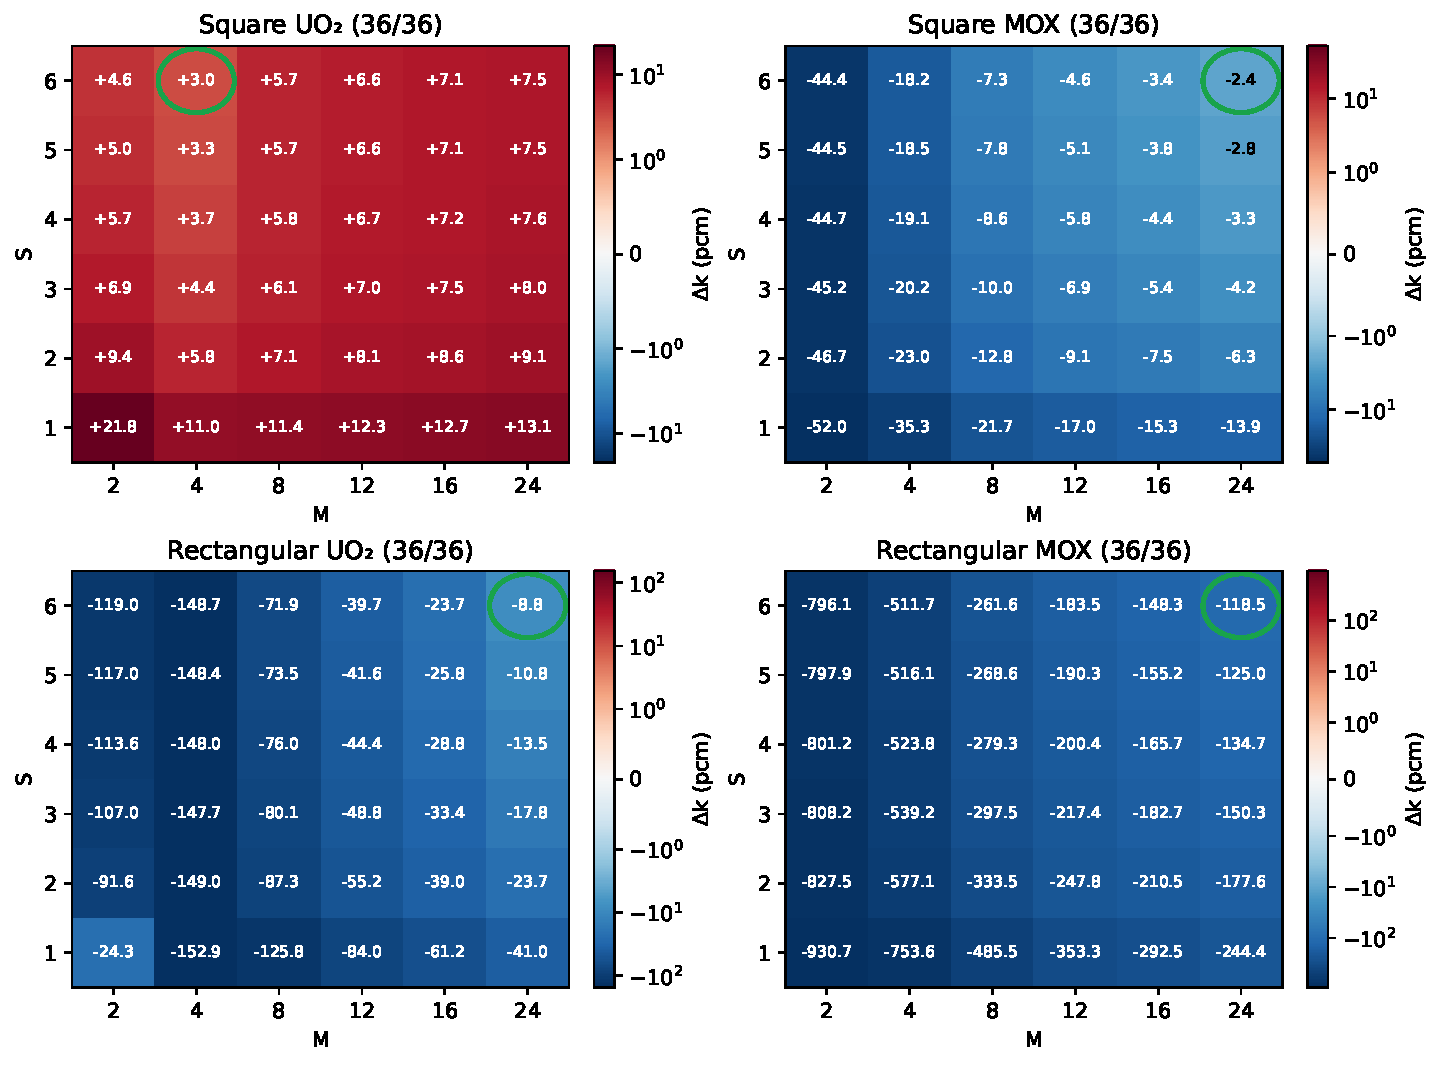
\includegraphics[width=.86\linewidth]{studyIII_c5g7_sm.pdf}
\caption{Signed eigenvalue differences for the pin-homogenised square and
explicit rectangular C5G7 assemblies, in pcm against each same-geometry
OpenMC reference. The marker indicates the smallest measured absolute
difference in each panel.}
\label{fig:study4-c5g7}
\end{figure}

\begin{figure}[htbp]
\centering
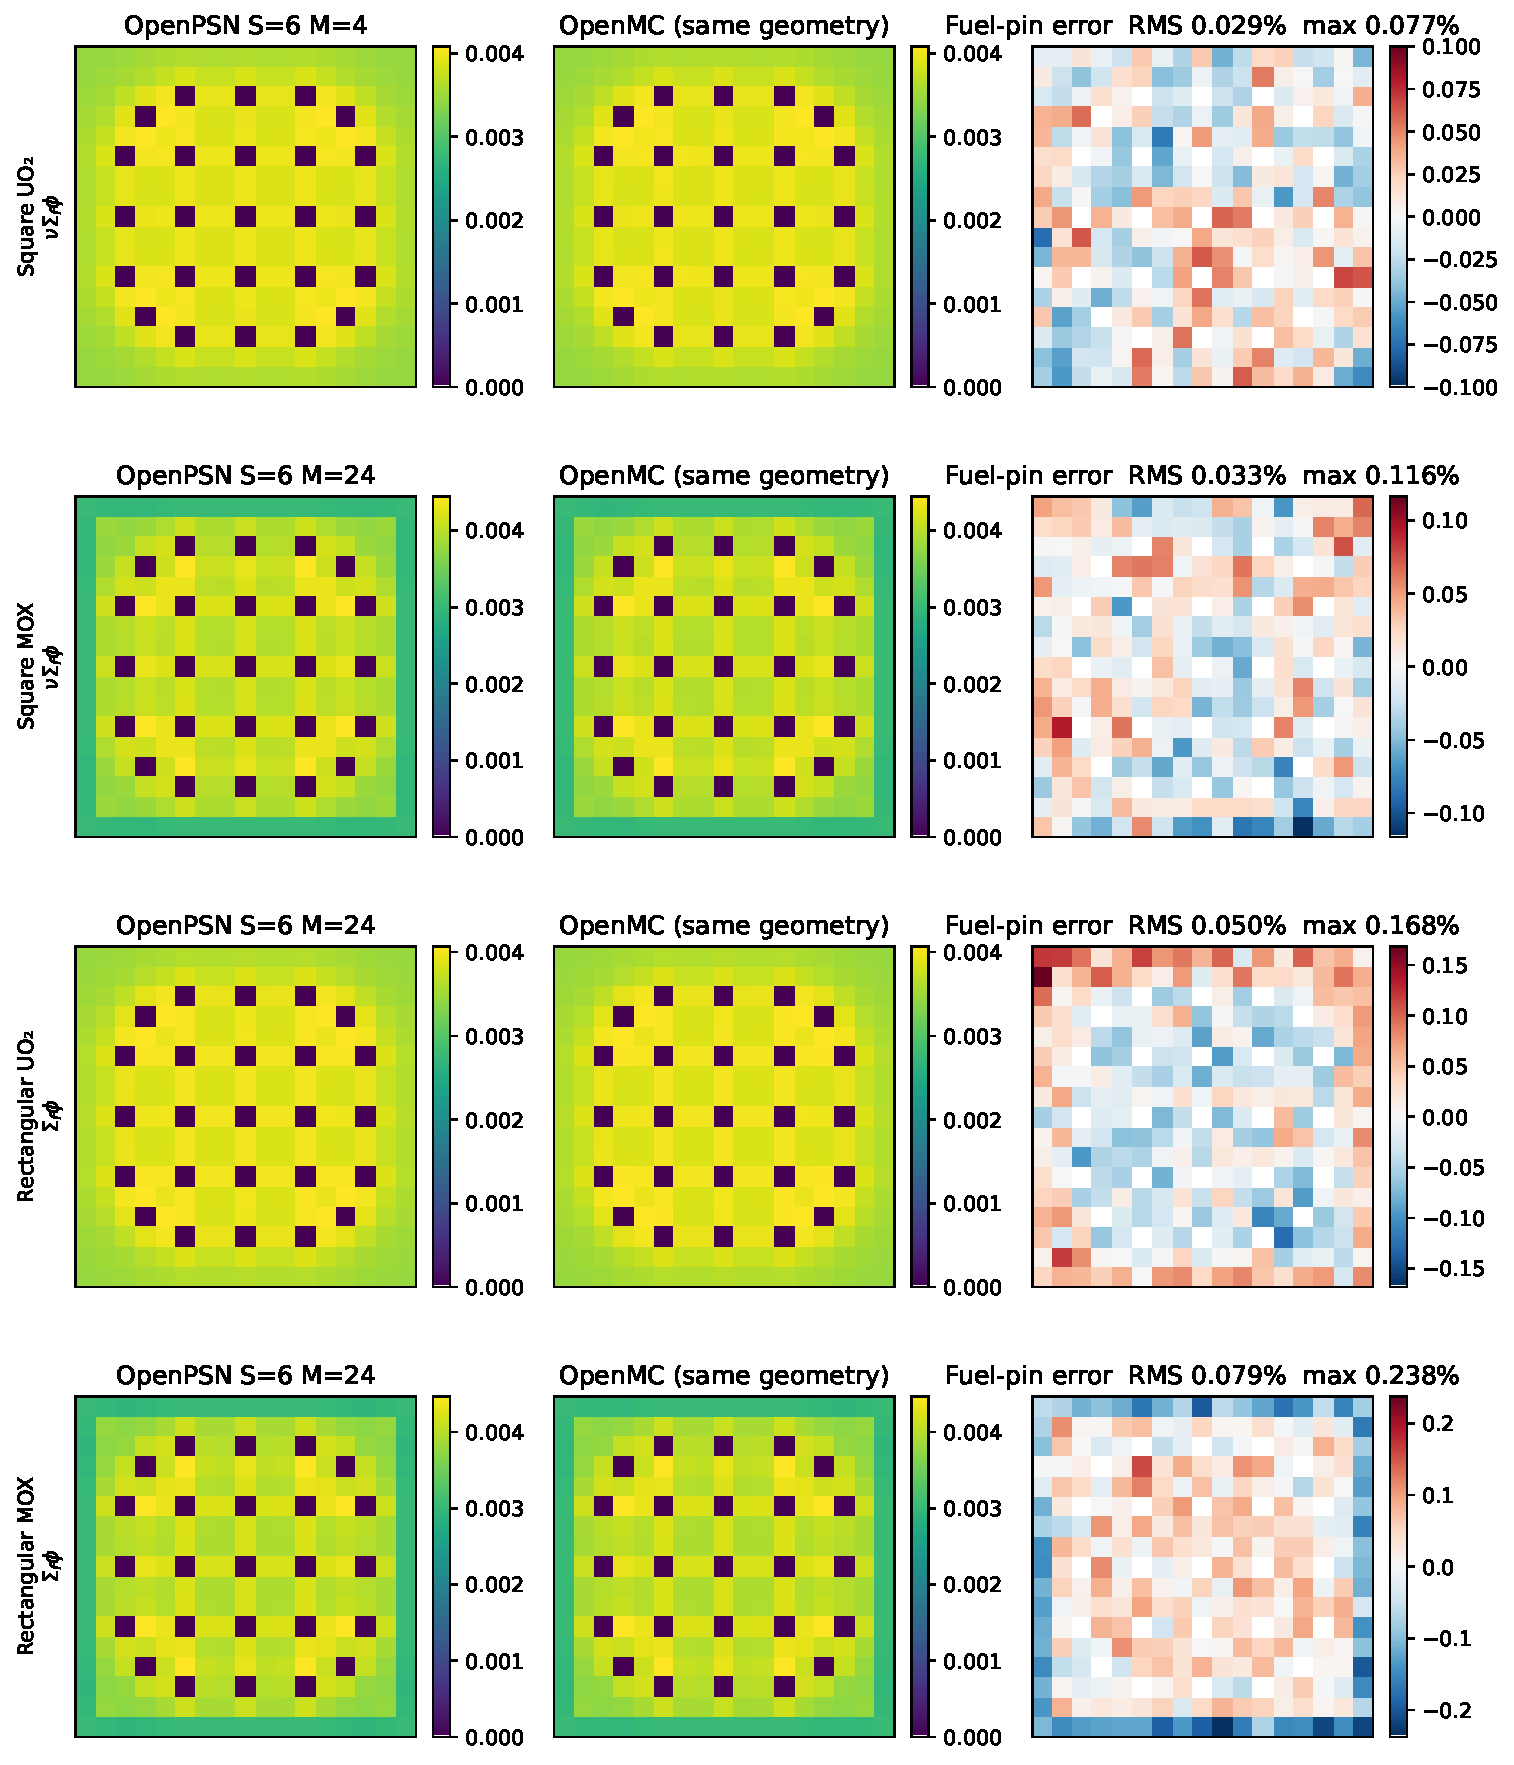
\includegraphics[width=.86\linewidth]{studyIII_best_fission.pdf}
\caption{Fuel-pin fission maps at the best measured points, from left to
right OpenPSN, OpenMC and the relative pin error. The square rows use
$\nu\Sigma_f\phi$, the rectangular rows $\Sigma_f\phi$, each normalised to
unit pin sum as in the corresponding Study I and II figures.}
\label{fig:study4-fission}
\end{figure}

\begin{table}[htbp]
\centering
\caption{Coverage, best measured point, fuel-pin error and wall time of the six $S\times M$ matrices, measured with the \texttt{sector\_average} closure at $A=1$. The sum column adds the individual point times; several cases ran concurrently on the same host.}
\label{tab:study4-assembly}
\centering\small
\begin{tabular}{l r r r r r}
\hline
Case & Best $(S,M)$ & $\Delta k$ (pcm) & Pin RMS & Pin max & Sum, 36--120 points\\
\hline
Strong absorber & $(20,24)$ & -33.67 & --- & --- & 140.1~s\\
Weak absorber & $(20,24)$ & -7.76 & --- & --- & 131.4~s\\
Square UO$_2$ & $(6,4)$ & +3.02 & 0.029\% & 0.077\% & 492.9~s\\
Square MOX & $(6,24)$ & -2.45 & 0.033\% & 0.116\% & 502.6~s\\
Rectangular UO$_2$ & $(6,24)$ & -8.80 & 0.050\% & 0.168\% & 3041.0~s\\
Rectangular MOX & $(6,24)$ & -118.55 & 0.079\% & 0.238\% & 2957.7~s\\
\hline
\end{tabular}
\end{table}


\begin{figure}[htbp]
\centering
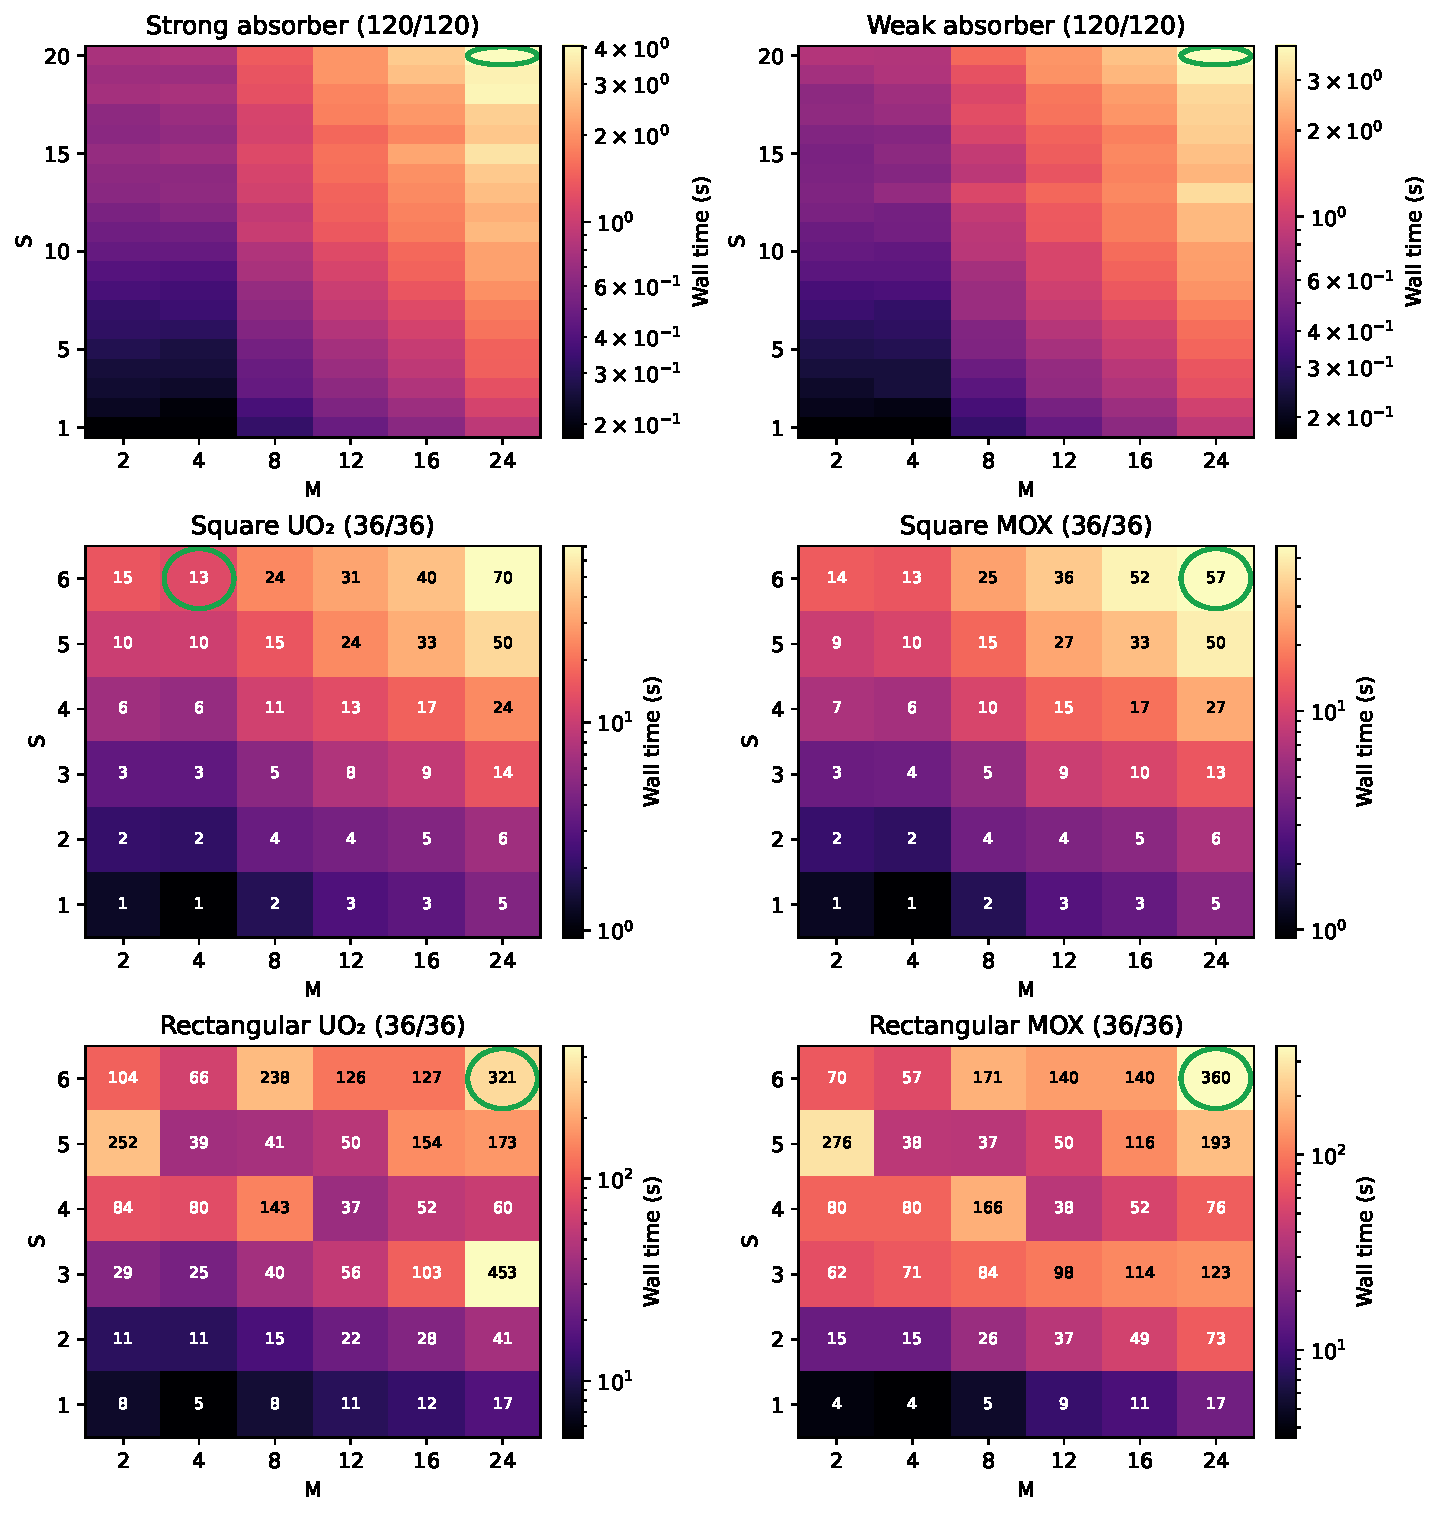
\includegraphics[width=.92\linewidth]{studyIII_wall_time.pdf}
\caption{End-to-end wall time of the same 384 points in seconds on a
logarithmic scale; top to bottom, strong and weak absorber checkerboards,
square UO$_2$ and MOX, rectangular UO$_2$ and MOX. Points were run several at
a time on one host and the coarse points take under a second, so the panels
describe workload rather than measured throughput.}
\label{fig:study4-walltime}
\end{figure}

The rectangular MOX row is the weakest point of this sweep, and it is a
material-and-tiling effect rather than an angular one: at fixed $M{=}24$,
$A{=}2$ and one polar mode, its error reduces from $-185.20\pcm$ at $S{=}1$
through $-115.02$ ($S{=}2$) and $-68.35$ ($S{=}4$) to $-52.81\pcm$ at
$S{=}6$, so spatial resolution of the explicit water gaps, not additional
azimuth, carries the improvement there.

The rectangular UO$_2$ matrices contain one non-monotone step that was
investigated separately. On the assembly mesh of the sweep row $S{=}2$, moving
from $M{=}2$ to $M{=}4$ makes the eigenvalue worse by $57.33\pcm$
($-91.65$ to $-148.98\pcm$). A change that does not touch the angular rule
reduces it: redistributing each pin's fixed cell budget among its three
material intervals (benchmark flag \texttt{--balance-pin}, which keeps the
three material boundaries and the total pin width and chooses the allocation
that minimises the widest subcell) brings the same paired step down to
$40.69\pcm$ ($-94.94$ to $-135.63\pcm$), and on the paired points it also
improves $M{=}4$, $8$ and $16$ for both materials: by $37.60$ and
$13.35\pcm$ at $M{=}4$, $36.63$ and $15.75\pcm$ at $M{=}8$, and $32.01$ and
$13.66\pcm$ at $M{=}16$, for MOX and UO$_2$ respectively, while the $M{=}2$
UO$_2$ point moves $3.29\pcm$ the other way. On the uniform
layout, raising the azimuth degree to $A{=}4$ with the higher spatial basis
gives $-71.17\pcm$ at $M{=}2$ and $-33.21\pcm$ at $M{=}4$, so the reversal
disappears there as well. The step is therefore an interaction between the
coarse sector and the coarse intra-pin spatial resolution, not a property of
the $M{=}4$ partition, and it is reduced by refining either side rather than
by an angular-rule change. Both controls are tabulated in
\texttt{paper/data/study4\_rectangular\_controls.csv} and
\texttt{paper/data/study4\_\allowbreak balance\_\allowbreak pin.jsonl}.

\paragraph{C5G7 rectangular quarter core.}
The $5\times6$ grid of runs on the explicit quarter core, with the direction-wise
\texttt{sector\_diffusion} closure
(\texttt{c5g7\_rect\_quarter\_core.yaml}, 7 groups, original interfaces,
$(153S)^2$ nodes, TY3 polar rule, $A{=}1$, 60-thread cap) is given in
Tables~\ref{tab:study4-core-pcm} and~\ref{tab:study4-core-time}. The
reference is the same-geometry OpenMC batch mean
$1.187217554586068$ with a $3.41\pcm$ standard error over
20{,}000 active batches; the statepoint \texttt{k\_combined} estimator is
$1.187220349151050$ with $1.75\pcm$. Each measured cell was solved independently and
re-verified by a separate transport sweep with a source residual of at most
$5\times10^{-9}$ and an eigenvalue residual of at most $10^{-9}$. Timings are
end to end for the recorded run and include assembly, factor construction,
outer iterations and the verification sweep; an asterisk marks a cell that
reused stored factors, and points sharing a time window were run concurrently,
so the two matrices describe workload as much as throughput.

\begin{table}[htbp]
\centering
\caption{Signed eigenvalue difference $10^{5}(\keff-k_\mathrm{ref})$ in pcm on the explicit quarter core, against the same-geometry OpenMC reference $1.187217554586$ ($3.41\,\mathrm{pcm}$ standard error). Bold marks the smallest measured absolute difference.}
\label{tab:study4-core-pcm}
\begin{tabular}{rrrrrrr}
\hline
 & \multicolumn{6}{c}{Azimuth sectors $M$}\\
\cline{2-7}
$S$ & 2 & 4 & 8 & 12 & 16 & 24\\
\hline
1 & -271.73 & -149.28 & -68.90 & -60.26 & -57.21 & -54.09 \\
2 & -263.55 & -137.20 & -49.66 & -40.31 & -37.10 & -33.95 \\
3 & -260.06 & -133.29 & -39.46 & -28.91 & -25.68 & -23.05 \\
4 & -257.30 & -131.26 & -33.57 & -22.58 & -19.44 & -16.77 \\
5 & -254.69 & -130.03 & -29.34 & -18.52 & -15.85 & \textbf{-12.98} \\
\hline
\end{tabular}
\end{table}

\begin{table}[htbp]
\centering
\caption{End-to-end wall time in seconds for the same points, including assembly, factor construction, outer iterations and the verification sweep. An asterisk marks a point that reused a stored factorisation. Points sharing a time window ran concurrently, so the column reports load rather than throughput.}
\label{tab:study4-core-time}
\begin{tabular}{rrrrrrr}
\hline
 & \multicolumn{6}{c}{Azimuth sectors $M$}\\
\cline{2-7}
$S$ & 2 & 4 & 8 & 12 & 16 & 24\\
\hline
1 & 77.8 & 113.4 & 166.4 & 176.1 & 237.8 & 340.7 \\
2 & 625.3 & 790.3 & 548.5 & 1299.0 & 996.6 & 1810.2 \\
3 & 1199.5 & 1757.3 & 1559.8 & 1787.4 & 2790.4 & 2518.8 \\
4 & 3263.4 & 1647.5 & 3486.0 & 2665.9 & 2163.1* & 4360.9 \\
5 & 5787.4 & 3161.0 & 3440.0 & 5084.0 & 4841.3* & 10930.6* \\
\hline
\end{tabular}
\end{table}


\begin{figure}[htbp]
\centering
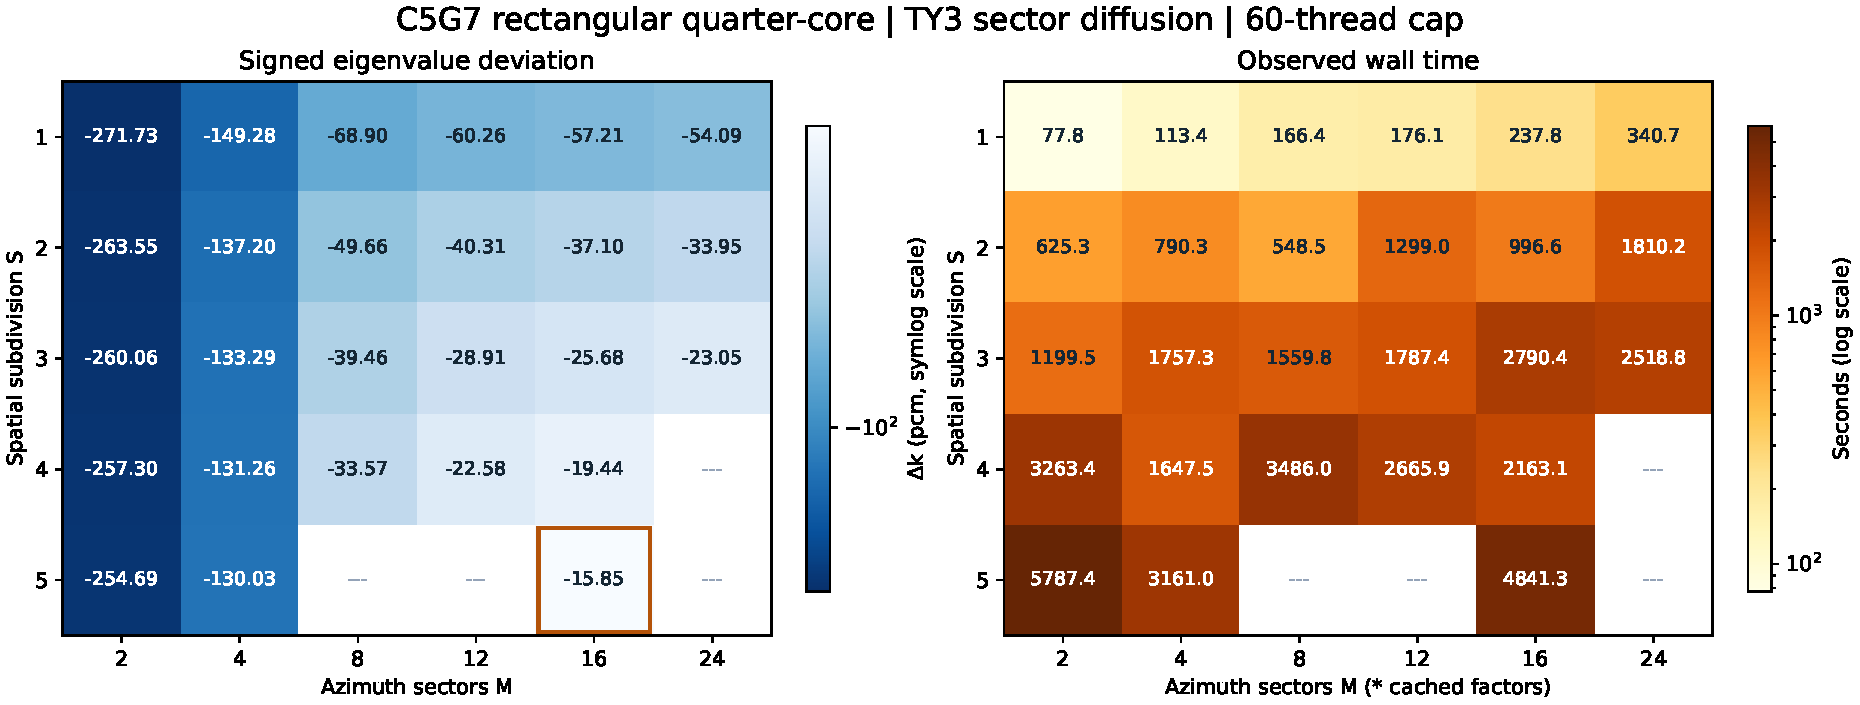
\includegraphics[width=\linewidth]{sector_diffusion_sm.pdf}
\caption{The measured quarter-core matrices. Left: signed eigenvalue
difference in pcm (symlog scale), the framed cell marking the smallest
absolute difference. Right: end-to-end wall time in seconds (log scale).}
\label{fig:study4-core}
\end{figure}

\begin{figure}[htbp]
\centering
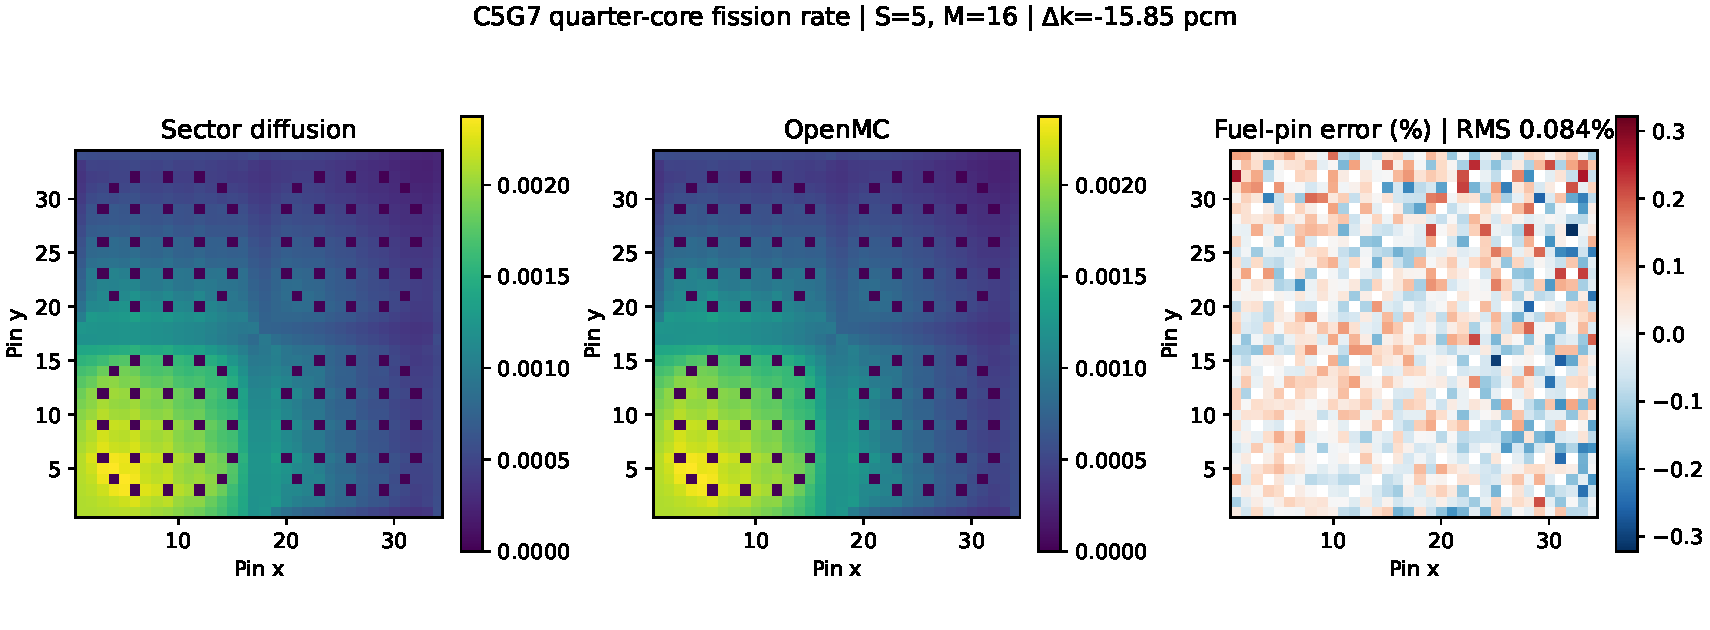
\includegraphics[width=\linewidth]{study4_core_fission.pdf}
\caption{Normalised fuel fission rate at the best measured quarter-core
point, beside the same-geometry OpenMC reference and the pin-wise relative
difference over the 1056 fuel pins.}
\label{fig:study4-core-fission}
\end{figure}

\begin{table}[htbp]
\centering
\caption{The cell of Table~\ref{tab:study4-core-pcm} with the smallest absolute
eigenvalue difference, with a relative pin-wise fission-rate difference of RMS 0.084\% and maximum absolute value 0.321\%. The node count is $(153S)^2$.}
\label{tab:study4-core-best}
\begin{tabular}{lr}
\hline
spatial subdivision $S$ & 5\\
azimuth sectors $M$ & 24\\
nodes & 585225\\
$\keff$ & 1.187087778706\\
$\Delta k$ & $-12.98\pcm$\\
wall time & 10930.6~s (stored factors)\\
\hline
\end{tabular}
\end{table}


For comparison on the identical geometry, grid and thread budget, starting
cold, the legacy PSN closure at $S{=}1$, $M{=}24$ gives $-10.12\pcm$ in
128.08~s and the sector closure $-54.09\pcm$ in 340.68~s. The sector closure
is therefore not uniformly better at the coarsest settings, where the legacy
node model has the smaller error at equal angular resolution; the tables above
show the sector error decreasing as either axis is refined, which is the
regime where the two paths cross.

One input-level effect is of the same size as these differences. OpenPSN
reads the C5G7 fission spectrum as supplied, with
$\sum_g\chi_g=1.00000917761$, whereas OpenMC renormalises it on read; the two
eigenvalues are related by $k_\text{raw}=(\sum_g\chi_g)\,k_\text{normalised}$,
which shifts the present reference by $1.0896\pcm$ --- the same order as the
stated target accuracy. Group-wise constant corrections of this kind are the
reason the comparison is reported cell by cell rather than as a single
number.

How far the remaining bias is azimuthal was estimated on the same base grid at
$I{=}8$ polar nodes and $A{=}1$: the successive increments
$M{=}4,8,16$ and $M{=}8,16,32$ give local azimuthal orders of $1.32$ and
$1.47$, and the two windows extrapolate to $-54.64\pcm$ and $-58.90\pcm$ as
$M\rightarrow\infty$ at fixed spatial and polar resolution. Space is not the
dominant partner either --- at fixed $M{=}16$, refining the $172\times172$
graded mesh to $244\times244$ moves $\keff$ by $3.24\pcm$. On this family of
meshes the residual difference is therefore limited by the intra-cell material
and polar resolution rather than by the number of azimuth sectors, and the
reference itself carries $3.39$--$3.91\pcm$ of statistical uncertainty (block
sizes of 10 to 500 batches, $1.75\pcm$ for the \texttt{k\_combined}
estimator), which is larger than the margin any single cell of
Table~\ref{tab:study4-core-pcm} would have to prove.

\paragraph{Symbolic and exact checks.}
Because the closure is now defined by an exact reduction, several of its
components were checked without discretisation. The two-layer vacuum slab with
unit optical depths and equilibrium source terms $1$ and $2$ has interface
scalar flux $3[1-E_2(1)]/2$, interface net current $-1/4+E_3(1)/2$, and
absorption plus leakage equal to the total source $3$; the reference
implementation reproduces these in rational arithmetic with exponential
integrals, and inserting a virtual interface or splitting the angular band
leaves every directional response and every per-cell balance unchanged. Substituting the analytic
flux into both the first-order transport equation and the even-parity second
order equation leaves a identically zero symbolic residual for a mirrored
rectangle with isotropic scattering, and the response coefficients of an
oblique characteristic crossing two interfaces and reflecting are unchanged
when extra spatial subdivisions are introduced. With the C5G7 cross sections
read as exact rationals, the four-reflection homogeneous seven-group
eigenvalues are $0.738214699120$ (UO$_2$) and $0.839334157439$,
$1.038903851962$, $1.147587627285$ (MOX 4.3\%, 7\%, 8.7\%). For the heterogeneous
quarter core, per-group weighted conservation verified with exact rational
linear programming certifies $k_\mathrm{eff}<1.894$; a bracket of the same width
as the target accuracy has not been obtained. These 14 exact checks (10 from
this round plus the 4 slab balances above) ship as
\texttt{examples/psn\_strict\_checks/} and run under \texttt{unittest
discover} in about 2~s with \texttt{sympy} and \texttt{PyYAML}; the
discretised operator, the node-response identity and the interface and symmetry
properties of the geometry controls are covered by the 22 regressions in
\texttt{tests/test\_sector\_diffusion.py}, which run in about 13~s. The exact
checks constrain the operator, not the truncation error of a production mesh.

\paragraph{Scope.}
The quarter-core matrix is a measured grid, not a convergence proof: its best
cell still differs from the Monte Carlo reference by more than that
reference's own $3.41\pcm$ standard error, the rectangular MOX assembly keeps
an order-of-tens-of-pcm bias at its best sampled setting, and the sector
closure is more expensive than the legacy path at equal $M$. What the
section establishes is narrower and checkable: with the face closure taken
from the same weak form as the body term, the sign-changing valley of the
square checkerboard does not appear anywhere in the 187 points of the
direction-wise closure of record except the single under-integrated
$A{=}1$, $M{=}4$ column, the error is one-signed outside it and decreases
under every refinement of the spatial axis, and on the paired points that
share $A$, $S$, $M$ and $I$ it is the smaller of the two closures at all but
five of them, at equal cost. The nodal-response rewriting is an exact
algebraic identity on the same discrete system, and the archived
cell-average scan of 130 points stays one-signed and monotone on both axes.
